%%%%%%%%%%%%%%%%%%%%%%%%%%%%%%%%%%%%%%%%%%%%%%%%%%%%%%%%%%%%%%%%%%%%%
% LaTeX Template: Project Titlepage Modified (v 0.1) by rcx
%
% Original Source: http://www.howtotex.com
% Date: February 2014
% 
% This is a title page template which be used for articles & reports.
% 
% This is the modified version of the original Latex template from
% aforementioned website.
% 
%%%%%%%%%%%%%%%%%%%%%%%%%%%%%%%%%%%%%%%%%%%%%%%%%%%%%%%%%%%%%%%%%%%%%%

\documentclass[12pt]{report}
\usepackage[a4paper]{geometry}
\usepackage[myheadings]{fullpage}
\usepackage{fancyhdr}
\usepackage{lastpage}
\usepackage{graphicx, wrapfig, subcaption, setspace, booktabs}
\usepackage[T1]{fontenc}
\usepackage[font=small, labelfont=bf]{caption}
\usepackage{fourier}
\usepackage[protrusion=true, expansion=true]{microtype}
\usepackage[english]{babel}
\usepackage{sectsty}
\usepackage{url, lipsum}
\usepackage{color}
\usepackage{hyperref}
\usepackage{array}
\usepackage{supertabular}
\usepackage{hhline}
\usepackage{enumitem}
\usepackage{graphicx}

\newcommand{\HRule}[1]{\rule{\linewidth}{#1}}
\renewcommand{\theenumii}{\arabic{enumii}.}
\addto\captionsenglish{
  \renewcommand{\contentsname}
    {Innhold}
}
\onehalfspacing
\setcounter{tocdepth}{5}
\setcounter{secnumdepth}{5}

%-------------------------------------------------------------------------------
% HEADER & FOOTER
%-------------------------------------------------------------------------------
\pagestyle{fancy}
\fancyhf{}
\setlength\headheight{15pt}
\fancyhead[L]{Team D} 
\fancyhead[R]{Universitetet i Bergen}
\fancyfoot[R]{Page \thepage\ of \pageref{LastPage}}
%-------------------------------------------------------------------------------
% TITLE PAGE
%-------------------------------------------------------------------------------

\begin{document}

\title{ \normalsize \textsc{}
		\\ [2.0cm]
		\HRule{0.5pt} \\
		\LARGE \textbf{\uppercase{Bilspill}}
		\HRule{2pt} \\ [0.5cm]
		\normalsize \today \vspace*{5\baselineskip}}

\date{}

\author{
		Team D  \\ 
		Universitetet i Bergen \\
		Informatikk }

\maketitle
\tableofcontents
\newpage

%-------------------------------------------------------------------------------
% Section title formatting
\sectionfont{\scshape}
%-------------------------------------------------------------------------------

%-------------------------------------------------------------------------------
% BODY
%-------------------------------------------------------------------------------

\section*{Bruksm{\o}nstertekst:}
\addcontentsline{toc}{section}{Bruksm{\o}nstertekst:}

\textbf{Tittel}: F� h�yest mulig score
\bigskip \\
\textbf{Akt{\o}rer}: �nspiller
\bigskip \\
\textbf{Prim{\ae}rakt{\o}r}: Spiller
\bigskip \\
\textbf{Tid}: Varierende, avhengig av spillers prestasjon
\bigskip \\
\textbf{M{\aa}l}: F� h�yest mulig highscore f�r man g�r tom for bensin
\bigskip \\
\textbf{Pre-conditions:} Spillet er startet p{\aa} en datamaskin

\subsubsection*{Hovedflyt:}
\begin{enumerate}
\item Spiller er i startmeny
\item Spiller starter spillet
\item Spiller styrer bil med venstre/ h�yre piltast
\item Spiller unng�r hindre
\item Spiller plukker opp mynter og bensin
\item Bil g�r tom for bensin, spillet stopper
\item Score og highscore vises
\item Spillet lagres
\item Tilbake til startmeny
\end{enumerate}

\pagebreak
\subsubsection*{Alternative handlinger:}

\begin{enumerate}[label=\Alph*]
\item 
\bigskip

\begin{enumerate}
\item @1 Spiller velger � oppgradere 
\item Spiller kj�per oppgraderinger
\item Bil blir bedre
\item Gjenoppta @1
\end{enumerate}
\item 
\bigskip

\begin{enumerate}
\item @1 Spiller trykker p� tannhjul-knapp
\item Spiller endrer innstillinger
\item Innstillinger lagres
\item Gjenoppta @1
\end{enumerate}
\item
\bigskip

\begin{enumerate}
\item @3 ,4,5 Spiller pauset spiller
\item Spiller kan enten avslutte eller fortsette
\item Dersom spiller velger � avslutte, hopp til @7
\end{enumerate}
\end{enumerate}

\pagebreak
\section*{Bruksm{\o}nsterdiagram:}
\addcontentsline{toc}{section}{Bruksm{\o}nsterdiagram:}

\vspace{4cm}
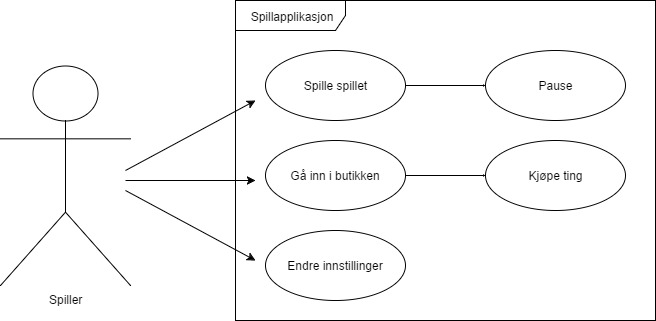
\includegraphics[width=0.8\textwidth,natwidth=500,natheight=642]{use_case_diagram_b.jpg}

\end{document}